\subsection{Reconstructing Importance Sampling Coreset}
As discussed in Section~\ref{sec:recover}, we use GANs to recover the data we lost while performing importance sampling. This was motivated from the observation that as we selected more number of points in importance sampling, the accuracy of the inference on the compressed data increased significantly (at times by $2\%$). Hence, the points which were not selected while performing importance sampling still had some importance and can be represented as a function containing the low level nuances of the activity performed and the sensor state. The challenge was to learn this function, i.e. to device a transformation function which can mimic the sensor signal given the aactivity and the sensor states. A similar problem, in terms of generating faces, paintings etc. given some latent space has already been solved using GANs~\cite{olszewski2017realistic}. Motivated by this, we designed a GANs to regenerate the lost data points while performing importance sampling. The latent space takes the activity, and the first and second order moments of the data sample to recreate the signal, and the Discriminator tried to distinguish between the generated signal and the actual signal. The generator is tuned repeatedly until the discriminator could not distinguish the original and the generated signal. The GAN modeled the lost signals with a very high correlation ($\ge 0.9$ in most cases and $0.6$ in some of the worst cases (refer Figure~\ref{Fig:gen} for an example). In rare cases (once in over 2000 cases), the generator induced artifacts which could result in wrong classifications. However, this error could be rectified with further fine tuning. 
% ; refer Figure~\ref{Fig:gen} for an example).

\subsection{More Results on Bearing Fault Data}
We repeated our experiments with similar experimental setup on the bearing fault data set~\cite{bearing}. The bearing fault data is sampled at a much higher frequency (48KHz) than the HAR data, and hence require a larger DNN, larger number of importance sampling, and more number of clusters. We took the learning from multiple domain specific literatures~\cite{bearing, eren2019generic, hoang2017convolutional} to isolate the frequency regions specific to the fault pattern to minimize the computations. But, because of the larger data volume, the number of computations performed at the edge diminished significantly (refer Figure~\ref{Fig:bComplete}). We also conducted an empirical study on number of clusters required, and found out that the bearing set data needs about 15 to 20 clusters to maintain the inference accuracy. The data volume communicated for different number of clusters is represented in Figure~\ref{Fig:bearingdata}. 

\begin{figure}
  \centering
  %\dummyfig{Sensor Setup}
  \includegraphics[clip,width=\linewidth]{figs/37.pdf}
  \caption{An example of generator based coreset recovery}
  \label{Fig:gen}
%\end{figure}
 \end{figure}

\begin{figure}
  \centering
  %\dummyfig{Sensor Setup}
  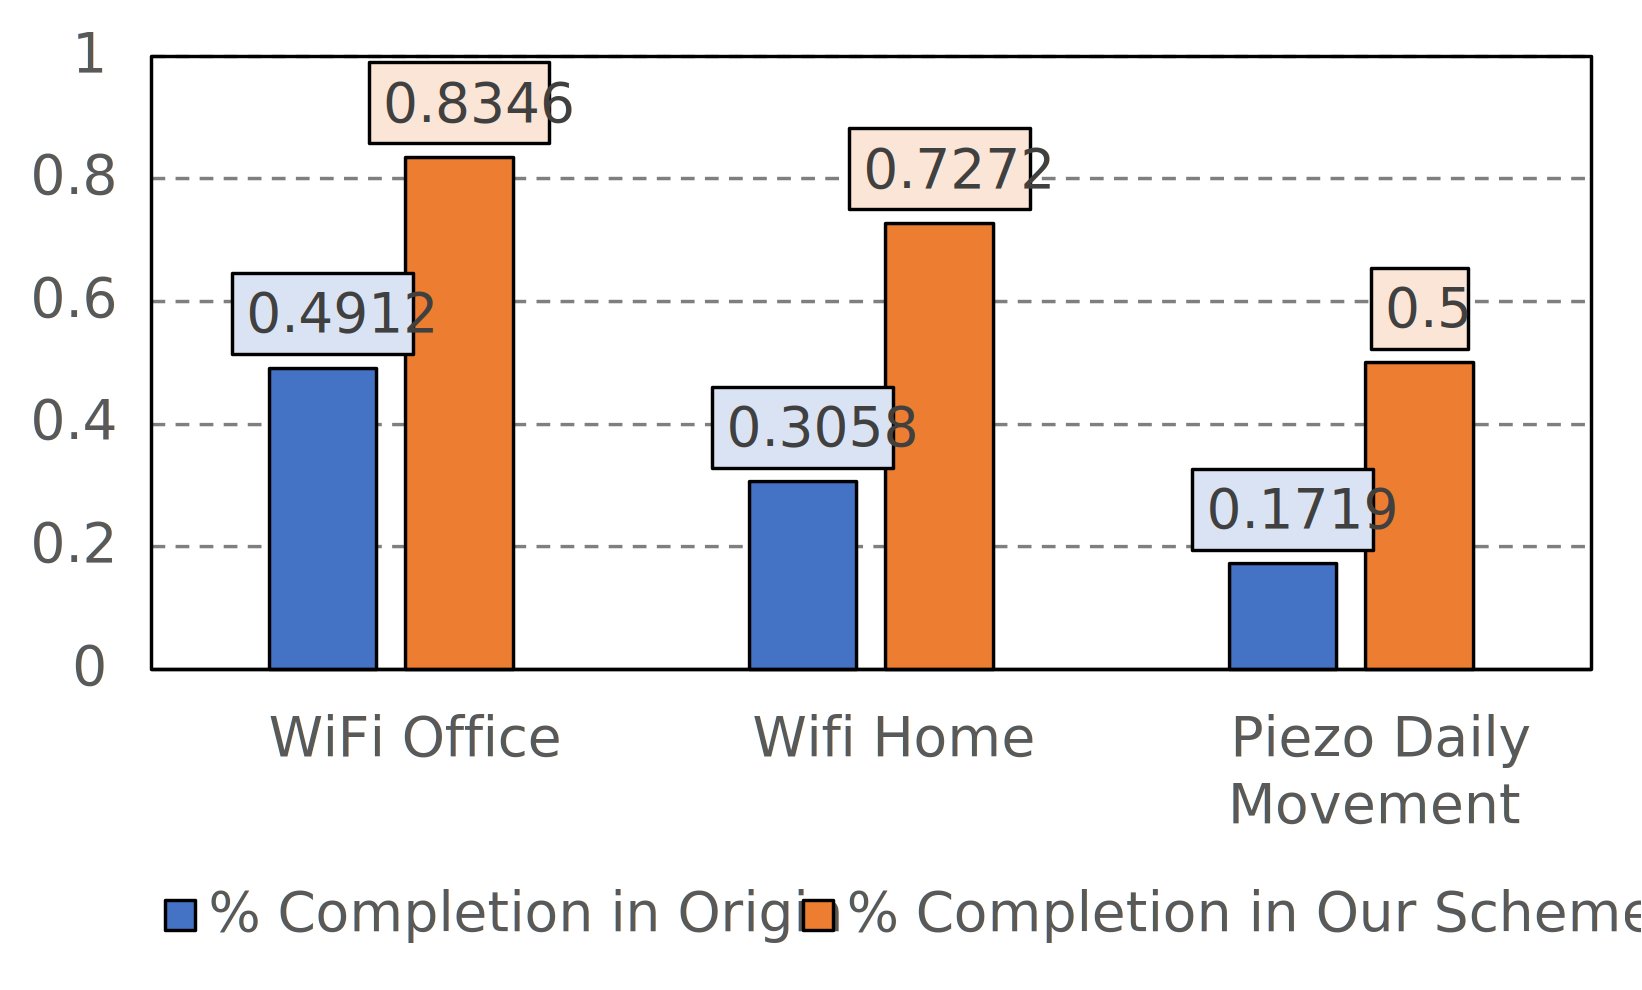
\includegraphics[clip,width=0.8\linewidth]{figs/bearingComp.png}
  \caption{\% completion of the inference at the edge for bearing fault data with different EH source.}
  \label{Fig:bComplete}
%\end{figure}
 \end{figure}


%%%%%%%%%%%%%%%%%%%%%%%%%%%%%%%%%%%%%%%%%%%%%%%%%%%%%%%%%%%%
 
 \begin{figure}
  \centering
  %\dummyfig{Sensor Setup}
  \includegraphics[clip,width=0.8\linewidth]{figs/bearingData.png}
  \caption{Communication data volume with different number of clusters.}
  \label{Fig:bCluster}
%\end{figure}
 \end{figure}

 \begin{table}
\centering
\resizebox{\linewidth}{!}{%
\begin{tabular}{|l|c|c|c|} 
\hline
Component & Spec & Power & Area(mm\textsuperscript{2}) \\ 
\hline
SRAM Buffers & \begin{tabular}[c]{@{}c@{}}1kB*256+\\8kB*256+\\64kB+16*256kB\end{tabular} & 10.372W & 117.164 \\ 
\hline
MAC Unit & \begin{tabular}[c]{@{}c@{}}(8*8)\\*256\end{tabular} & 8.46W & 32.72 \\ 
\hline
\begin{tabular}[c]{@{}l@{}}Adder Tree and \\Comparator\end{tabular} & 16*16bit + 256 & 2.4W & 21.556 \\ 
\hline
Control & -- & 0.96W & 12.2 \\ 
\hline
Host & $\sim$Cortex A78 series & 11W & -- \\ 
\hline
\multicolumn{4}{|c|}{Design at 592MHz with~Synopsys AED 32nm library} \\ 
\hline
\multicolumn{1}{|c|}{\textbf{Total}} & 256 tiles & 33.192W & 183.64 \\
\hline
\end{tabular}
}
\vspace{-4pt}\caption{Area and power estimation of our design.}
\label{tab:specs}
\vspace{-14pt}
\end{table}

%%%%%%%%%%%%%%%%%%%%%%%%%%%%%%%%%%%%%%%%%%%%%%%%%%%%%%
\begin{figure*}[ht]
\centering
    \subfloat[Accuracy with MHEALTH dataset]
    {
    \includegraphics[width=0.48\linewidth
    , height=2.5cm
    ]{figs/8.pdf}\label{Fig:MHEALTH-accuracy}
    }
    \hfill
    \subfloat[Accuracy with PAMAP2 dataset]
    {
    \includegraphics[width=0.48\linewidth
    , height=2.5cm
    ]{figs/9.pdf}\label{Fig:PAMAP-accuracy}
    }
\caption{Accuracy and communication efficiency of \emph{Seeker} with different data sets and sensitivity study.}
    %\vspace{-0.1cm}
    \label{fig:AllAccuracy}  
    %\vspace{-0.5cm}
\end{figure*}
%%%%%%%%%%%%%%%%%%%%%%%%%%%%%%%%%%%%%%%%%%%%%%%%%%%%%%